% !TEX root = ../fib_poly.tex

\section{Diagonals} \label{s:diagonals}

\todo{@anibal: Intro to \cref{s:diagonals}}

\subsection{Diagonals polytope}

\begin{figure}[b]
	\centering
	% !TEX root = ../fib_poly.tex

\begin{figure}[h!]
\centering
\resizebox{0.7\linewidth}{!}{
\begin{tikzpicture}[>=stealth]

\path[<-] (3.5,0)node[right]{$ $} edge(-1,0) (0,3)node[above]{$ $} edge(0,-1);

\node at(0,-0.01){$\bullet$};

\node at(-0.25,-0.25){$0$};

\node at(2,-0.01){$\bullet$};

\draw[thick] (0,0)--(2,0);

\node at(2.25,-0.25){$1$};

\end{tikzpicture}
\quad \resizebox{0.05\linewidth}{!}{\raisebox{3em}{$\longrightarrow$}} \quad \quad
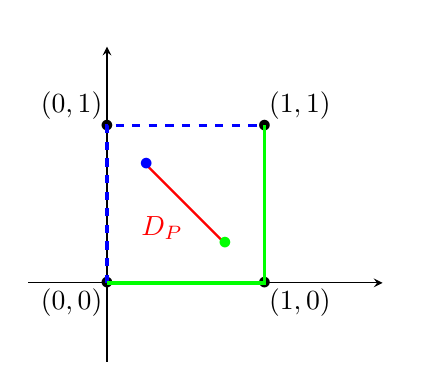
\begin{tikzpicture}[>=stealth]

\path[<-] (3.5,0)node[right]{$ $} edge(-1,0) (0,3)node[above]{$ $} edge(0,-1);

\node at(0,-0.01){$\bullet$};

\node at(-0.45,-0.25){$(0,0)$};

\node at(2,-0.01){$\bullet$};

\node at(2.45,-0.25){$(1,0)$};

\node at(2,2-0.01){$\bullet$};

\node at(2.45,2.25){$(1,1)$};

\node at(0,2-0.01){$\bullet$};

\node at(-0.45,2.25){$(0,1)$};

\draw[thick] (0,0)--(2,0)--(2,2);

\draw[thick, red] (0.25*2,0.75*2)--(0.75*2,0.25*2);

\node at(0.5,1.5){\color{blue}$\bullet$};

\node at(1.5,0.5){\color{green}$\bullet$};

\node at(0.7,0.7){\color{red}$D_P$};

\draw[very thick, blue,dashed] (0,0)--(0,2)--(2,2);
\draw[very thick, green] (0,0)--(2,0)--(2,2);

\end{tikzpicture}}
\caption{The polytope of diagonals of the interval (in red). Its two vertices define cellular approximations of the diagonal (dashed, in blue, and in green).}
\label{figure:cellularapproximation}
\end{figure}
	\caption{The polytope of diagonals of the interval (in red). Its two vertices define cellular approximations of the diagonal (dashed, in blue, and in green).}
	\label{figure:cellularapproximation}
\end{figure}

\begin{definition}
	The \emph{diagonals polytope} $D_P$ of a polytope $P$ is the fiber polytope of the projection
	\[
	\begin{tikzcd}[row sep=-2,column sep=small]
		P \times P \arrow[r] & P \\
		(x,y) \arrow[r,mapsto] &\textstyle\frac{x+y}{2}.
	\end{tikzcd}
	\]
\end{definition}

We observe that $P$ embeds into $P\times P$ via the set-theoretic diagonal $\Delta (x)=(x,x)$, which is a section of $\pi$.
The vertices of $D_P$ are associated with tight coherent sections, which are cellular approximations of the diagonal $\Delta$ by \cite[Proposition 5]{MTTV19}, see also \cite[Proposition 1.1]{GLA21}.

\begin{example} \label{e:permutahedron}
	If $P=\sum_{1 \leq i<j \leq n+1} [e_i-e_j, e_j-e_i]$ is the standard $n$-dimensional permutahedron, then $D_P$ is the zonotope $\sum_{I<J} [\sum_{i \in I}e_i - \sum_{j \in J}e_j, \sum_{j \in J} e_j - \sum_{i \in I}e_i]$, where the sum runs over all pairs $I,J\subset [n+1]$ such that $|I|=|J|\neq 0, I\cap J = \emptyset$ and $\min(I \cup J) \in I$, see \cite[Theorem 3.6]{GLA21}.
\end{example}

\subsection{Tangent-Normal isomorphism}

Consider the diagonal embedding
\[
\begin{tikzcd}[row sep=0, column sep=small]
	\Delta \colon \R^n \arrow{r} & \R^n \times \R^n \\
	\phantom{\Delta \colon} z \arrow[r, |->] & (z,z) \ ,
\end{tikzcd}
\]
and denote by $\{e_j\}$ the standard basis of $\R^n$.
Then, $\{\Delta (e_j)\}$ is a basis of $\Ima \Delta$ and we have an isomorphism $\R^n \cong \Ima \Delta$.
A basis for the orthogonal complement $\Ima \Delta^{\bot}$ is $\{(e_j,-e_j)\}$, and we have an isomorphism $\R^n \cong \Ima \Delta^{\bot}$.
For any $z \in \R^n$, we have $\pi^{-1}(z)=\Delta(z)+\ker \pi$, and an affine isomorphism
\begin{equation} \label{eq:D_P-iso}
	\begin{matrix}
		\iota_z & : & \R^n & \cong & \pi^{-1}(z) \\
		& & v & \mapsto & \Delta(z)+(v,-v).
	\end{matrix}
\end{equation}
The polytope of diagonals $D_P$ has the same dimension as $P$, and can be seen in $\R^n$ via the isomorphism $\iota_0$.

\begin{remark}
	We can see this isomorphism as the discrete analogue of the isomorphism between the tangent bundle of a manifold $M$ and the normal bundle of the diagonal submanifold of $M\times M$.
\end{remark}

We can also see that the normal fan of $D_P$, seen in the same space as $P$ under the isomorphism $\iota_0$, refines the normal fan of $P$.
Moreover, the \emph{fundamental hyperplane arrangement} of $P$, introduced in \cite[Definition 1.18]{GLA21}, is obtained from the normal fan of $D_P$ by extending all the walls to hyperplanes.
In the case where the normal fan of $D_P$ is already an hyperplane arrangement (for example, when $D_P$ is a zonotope, or when $P$ is a zonotope), it then agrees with the fundamental hyperplane arrangement of $P$.

\subsection{Reflections and fibers}

\todo{@guillaume: consider making this discussion have no lemmas and proofs}

We denote by $\rho_z P \defeq 2z-P$ the reflection of $P$ with respect to $z \in P$.

\begin{lemma}
	There is an affine isomorphism
	\begin{equation} \label{eq:iso-intersection}
		\begin{matrix}
			\rho \colon & & P \cap \rho_z P & \xra{\cong} & \pi^{-1}(z) \\
			& & x & \mapsto & (x,2z-x)
		\end{matrix}
	\end{equation}
	for all $z \in P$.
	\anibal{Do you need the name of the map ``$\rho$''?}
\end{lemma}

\begin{proof}
	This is a straightforward observation.
	Equivalently, the isomorphism can be given by the assignment $z+t \mapsto (z+t,z-t)$.
\end{proof}

This lemma makes clear the pointwise description of the diagonal
\begin{equation*}
	\begin{matrix}
		\triangle_{(P,v)} & : & P & \to & P \times P \\
		& & z & \mapsto & (\bm_v(P \cap \rho_z P),\tp_v(P \cap \rho_z P))
	\end{matrix}
\end{equation*}
in \cite[Definition 10]{MTTV19}, see also \cite[Proposition 1.15]{GLA21}.
Indeed, the tight coherent section associated to a vertex in $D_P$ is given by the extremal vetices of all the fibers $\pi^{-1}(z), z \in P$ with respect to some functional $\angles{-,w}$.
Since $D_P \subset \ker \pi$, we can restrict ourselves to the vectors of the form $w=(v,-v) \in \ker \pi$ without loosing generality.
Under the isomorphism (\ref{eq:iso-intersection}) above, we see that the maximum (resp. minimum) of $(v,-v)$ over $\pi^{-1}(z)$ is exactly the top (resp. bot) element of $P\cap \rho_z P$ with respect to $v$.

\subsection{Symmetry}

\begin{lemma}
	For any polytope $P$, the polytope of diagonals $D_P$ is centrally symmetric.
\end{lemma}

\begin{proof}
	Let $x = (y,-y)$ be a vertex of $D_P$.
	There is a linear form $\angles{-,v}$ which is maximized at $x$ over $D_P$.
	Its associated tight coherent section
	\begin{equation*}
		\begin{matrix}
			\gamma & : & P & \to & P \times P \\
			& & x & \mapsto & (\gamma_1(z),\gamma_2(z))
		\end{matrix}
	\end{equation*}
	is given by maximum of $\angles{-,v}$ in each fiber $\pi^{-1}(z)$ of $\pi$.
	Then, the section
	\begin{equation*}
		\begin{matrix}
			\sigma_2\gamma & : & P & \to & P \times P \\
			& & x & \mapsto & (\gamma_2(z),\gamma_1(z))
		\end{matrix}
	\end{equation*}
	is given by the minimum of $\angles{-,v}$ in each fiber, or equivalently the maximum of of $\angles{-,-v}$ in each fiber.
	Thus, this tight coherent section defines a vertex $-x=(-y,y)$ of $D_P$.
\end{proof}

\todo{@guillaume: Maybe explain the action... reversing .... corresponds to ... and to ...}

\subsection{Steenrod diagonals}

%\begin{definition}
%	A \emph{Steenrod diagonal} on $P$ is the datum of a frame which possess the bot-top property with respect to $D_P$.
%\end{definition}
%
%Observe that a Steenrod diagonal of $P$ defines a Steenrod diagonal on every face of $P$.
%\anibal{Why?}

%\anibal{Do you mean $D_P$ here?}
%According to \cref{ss:centrally-symmetric}, the iterated fiber polytope of $P$ is a family of centrally symmetric polytopes.
%Moreover, \cref{ss:zonotopes} shows that if $P$ is a zonotope, then the iterated fiber polytope of $P$ is a family of centrally symmetric zonotopes.
%\Guillaume{check:the product of zonotopes is a zonotope}

\begin{definition}
	A Steenrod diagonal on $P$ is an $\Sym_2$-equivariant topological, piecewise linear, cellular map $I^\infty \times P \to P \times P$.
\end{definition}

\todo{@guillaume: I think there should be a general adjunction construction starting with a piecewise linear map $R \to \Sigma(P,Q)$ and producing a piecewise linear map $R \times P \to Q$. I would include that construction on the section on framed polytopes.}

\begin{theorem}
	Let $(P,\{v_i\})$ be a framed polytope.
	If $(D_P, \{(v_i,-v_i)\})$ has the bot-top property then
	$(P,\{v_i\})$ has a canonical Steenrod diagonal.
\end{theorem}

\begin{proof}
	From \cref{ss:globularization} we get a family of $\Sym_2$-equivariant cellular maps
	\[
	\triangle_k, \triangle_k^\op : I^k \to D_P \ .
	\]
	The maps $\triangle_0, \triangle_0^\op$ select two vertices of $D_P$, that is two tight coherent sections of $P\times P \xra{\pi} P$ that we still denote by $\triangle_0, \triangle_0^\op : P \to P\times P$.
	Similarly the vertices in the polytopal subdivision of the source $I$ of the maps $\triangle_1$ and $\triangle_1^\op$ are sent to tight coherent sections of $\pi$.
	Thus, the two maps $\triangle_1$ and $\triangle_1^\op$ define discrete coherent homotopies
	\[
	\triangle_1, \triangle_1^\op : I\times P \to P \times P
	\]
	between these the sections $\triangle_0$ and $\triangle_0^\op$.
	The higher maps are obtained in a similar fashion, the ones above the dimension of $P$ being trivial.
\end{proof}

\subsection{Other stuff to be worked out}

\begin{lemma} \label{l:bot-top-for-DP}
	Let $\{v_k\}$ be an orthogonal basis of $\R^n$, and let $P\subset \R^n$ be a polytope.
	Then, we have that
	\[
	(D_P,\{v_k\}) \text{ has the bot-top property (resp. } \{v_k\} \text{ is }D_P\text{-admissible)}
	\]
	\[
	\iff (P\cap \rho_z P,\{v_k\}) \text{ has the bot-top property (resp. } \{v_k\} \text{ is }P\cap \rho_z P\text{-admissible)} \ \forall z \in P \ .
	\]
\end{lemma}

Note that we make a slight abuse of notation on the left-hand side, denoting by $D_P$ the inverse image $\iota_0^{-1}(D_P)$ of the polytope of diagonals under the isomorphism~(\ref{eq:D_P-iso}).

\begin{proof}
	Using the isomorphism (\ref{eq:D_P-iso}), it suffices to prove the statement for $(D_P,\{v_k,-v_k\})$ and $\pi^{-1}(z), z \in P$, which is a special case of \cref{t:bot-top-for-fibers}.
\end{proof}

\begin{theorem}
	If $(D_P,\{v_k\})$ has the bot-top property, then $\{v_k\}$ is $P$-admissible.
\end{theorem}

\begin{proof}
	Suppose that $(D_P,\{v_k\})$ has the bot-top property.
	Using \cref{l:bot-top-for-DP}, this is equivalent to $(P\cap\rho_z P, \{v_k\})$ having the bot-top property for all $z \in P$.
	On the other hand, by \cref{l:bot-top-admissible} it suffices to show that $\{v_k\}$ is $F$-admissible, for any face $F$ of $P$.
	Thus, we only need to show that if $(F \cap \rho_z F, \{v_k\})$ has the bot-top property, for all $z \in F$, then $(F,\{v_k\})$ has the bot-top property.

	For an edge $F_1$ of $P$, the two conditions are equivalent since $F_1 \cap \rho_z F_1 = F_1$, for $z$ the middle point between the vertices of $F_1$.
	For a $2$-face $F_2$ of $P$, we first have that every edge of $F_2$ is oriented by $v_1$, which implies that the intersection of $F_2$ with any hyperplane perpendicular to $v_1$ is a line $\ell$ (except for $\bm_{v_1}(F_2)$ and $\tp_{v_1}(F_2)$) with two distinct vertices $x$ and $y$ that belong to two distinct edges of $F_2$.
	Choosing $z \defeq (x+y)/2$, we have that if $F_2 \cap \rho_z F_2$ has the bot-top property with respect to $v_2$, then the line $\ell$ has the bot-top property, or equivalently is oriented by $v_2$.
	Thus, all such lines are oriented by $v_2$, and the frame $\{v_k\}$ is $F_2$-admissible.
	Continuing the induction process in the same fashion, we obtain that this is the case for any face $F$ of $P$.
\end{proof}

\begin{example}
	Note that the reverse implication in the preceding proposition does not hold in general.
	For instance, the standard $3$-dimensional permutahedron $P$ is oriented by the vector $v_1=(4,3,2,1)$, while the intersection $F \cap \rho_z G$, for $F$ and $G$ the faces associated to the ordered partitions $12|34$ and $24|13$, does not have the bot-top property with respect to $v_1$, for any $z \in (\mathring F + \mathring G)/2$.
	This is due to the fact that $v_1$ lies in one of the hyperplanes in the normal fan of $D_P$, see \cref{e:permutahedron}.
\end{example}

\Guillaume{Conjecture: the reverse implication holds for the simplices and cubes}

\Guillaume{Fundamental hyperplane arrangement gives combinatorial description of Steenrod diagonal?}

We turn our attention to the special case where $P = \gsimplex^n$, the standard $n$-simplex.

\begin{lemma}
	The polytope of diagonals $D_{\gsimplex^n}$ of the standard $n$-simplex is the $n$-dimensional permutahedron.
\end{lemma}

\begin{lemma}
	The frame ... defines a Steenrod diagonal on $\gsimplex^n$.
\end{lemma}

\begin{theorem}
	This choice recovers both Steenrod original construction, and Street orientals.
\end{theorem}

This provides a topological enhancement of the results...

\Guillaume{moduli space of Steenrod diagonals}

\Guillaume{unicity for simplices}


